The critical step in applying the change of variable formula is solving the relationship between $R_0$ and $p$ for $p$ and taking the derivative with respect to $R_0$ (using a dummy variable) as follows:

\begin{align*}
    f_Y(y) &= \left|\frac{d}{dy}h(y)\right|f_X(h(y))\\
    f_{R_0}(o) &= \left|\frac{d}{do}h(o)\right|f_p(h(o))\\
    &= \left|\frac{d}{do}\frac{r}{o+r}\right|f_p(p)\\
    &= \left|\frac{-r}{(o+r)^2}\right|f_p(p)\\
    P(R_0|X,r=5) &= \left|\frac{-5}{(R_0+5)^2}\right|P(p|X,r=5)
\end{align*}

\begin{figure}[H]
    \centering
    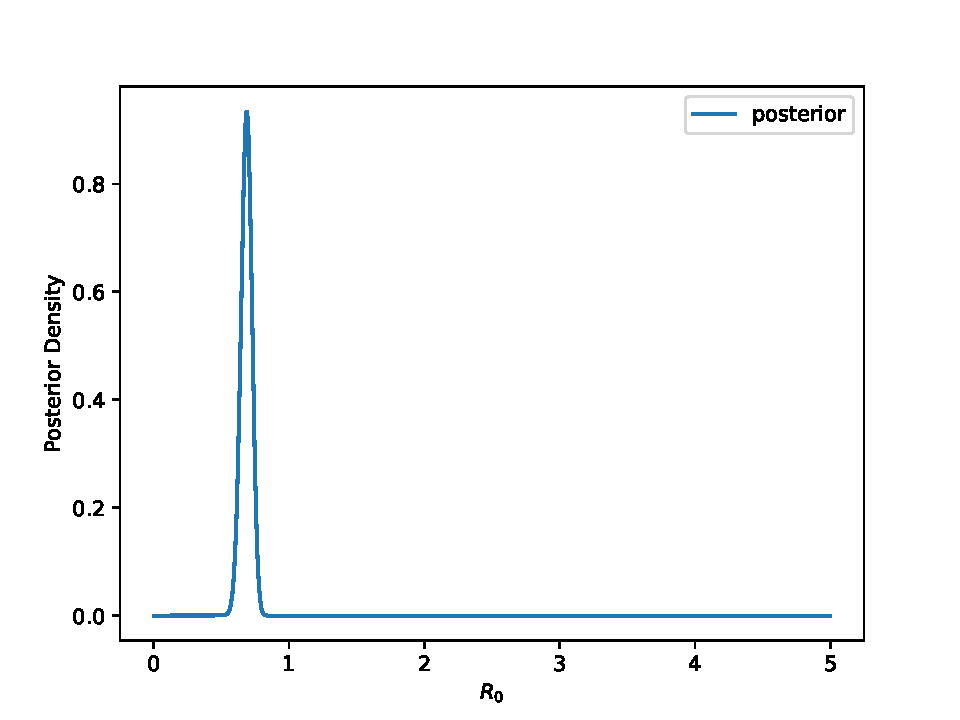
\includegraphics[width=0.8\linewidth]{images/r0_posterior_density.pdf}
    \caption{Posterior density for $R_0$. $R \in (0, \infty)$; 5 is arbitrarily chosen.}
    \label{fig:r0density}
\end{figure}


$R_0$ is clearly $<1$, which means this outbreak is unlikely to carry on.